% "{'classe':('PSI'),'chapitre':'cin_geo','type':('td','todo'),'titre':'Tête de découpe de tissus', 'source':'CCP MP 2018','comp':(''),'corrige':True}"
%\setchapterimage{fig_00.jpg}
\chapter*{Application \arabic{cptApplication} \\ 
Tête de découpe de tissus -- \ifprof Corrigé \else Sujet \fi}
\addcontentsline{toc}{section}{Application \arabic{cptApplication} : 
Tête de découpe de tissus -- \ifprof Corrigé \else Sujet \fi}

\iflivret \stepcounter{cptApplication} \else
\ifprof  \stepcounter{cptApplication} \else \fi
\fi


\marginnote[1cm]{
%\UPSTIcompetence[2]{B2-14}
%\UPSTIcompetence[2]{C1-05}
%\UPSTIcompetence[2]{C2-07}
}

\marginnote{CCP MP 2018}

\begin{marginfigure}
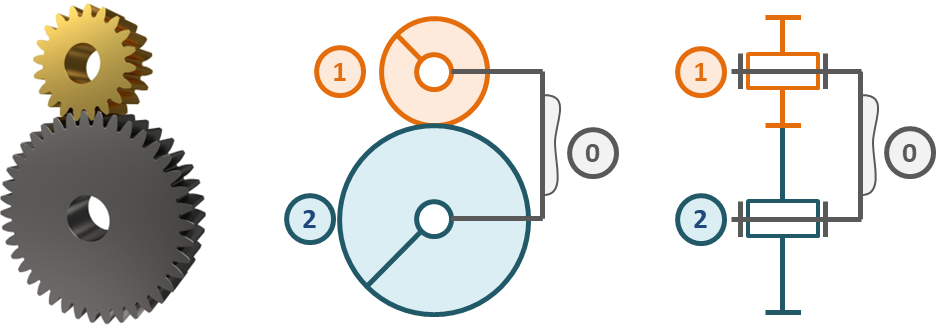
\includegraphics[width=\linewidth]{fig_01.png}
\end{marginfigure}




\subsection*{Présentation du système}
\ifprof
\else
Le système étudié dans ce sujet est une tête de coupe de tissus conçue et réalisée par la société
française Lectra, leader mondial dans la découpe automatisée des tissus.
Un système de découpe automatisé de tissus est composé :
\begin{itemize}
\item d'une table de découpe sur laquelle le tissus à découper (appelé matelas) est maintenu en position
par aspiration ;
\item d'un bras transversal qui se déplace en translation de direction $\vect{y_0}$ par rapport à la table ;
\item d'une tête de coupe qui se déplace en translation de direction $\vect{x_0}$ par rapport au bras transversal ;
\item d'un ordinateur qui pilote l’ensemble du système. 
\end{itemize}

\begin{marginfigure}
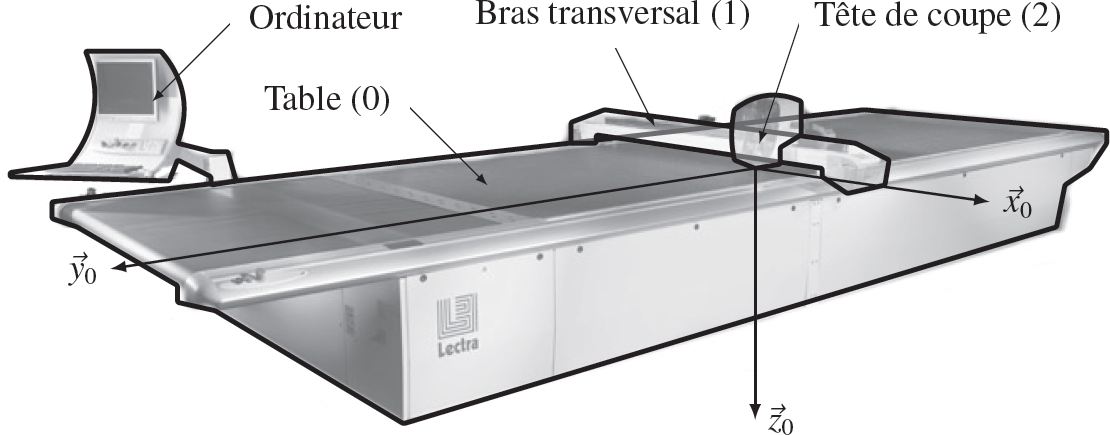
\includegraphics[width=\linewidth]{fig_02}
\end{marginfigure}

\fi

\begin{obj}
Déterminer la loi entrée/sortie de la chaîne cinématique de la tête de coupe et valider son
comportement vis-à-vis des exigences :
\begin{itemize}
\item 1.2.2.3 : la lame doit se déplacer d'une amplitude minimale de $\SI{20}{mm}$;
\item 1.2.2.4 : la vitesse de coupe maximale doit être de \SI{4}{m.s^{-1}} à $\pm\,5\,\%$. 
\end{itemize}
\end{obj}

\subsection*{Modélisation du comportement de la tête de coupe}

La découpe du tissu est réalisée par un mouvement de translation alternative d’une lame par rapport
au matelas de tissus. Ce mouvement est obtenu par un système bielle-manivelle dont le schéma cinématique
est donné à la figure suivante. Les mouvements de translation de la tête de coupe par rapport à la
table impliquent que les bases $\base{x_2}{y_2}{z_2}$ et $\base{x_0}{y_0}{z_0}$, liées respectivement à la tête de coupe et à la table, sont identiques.

\begin{marginfigure}
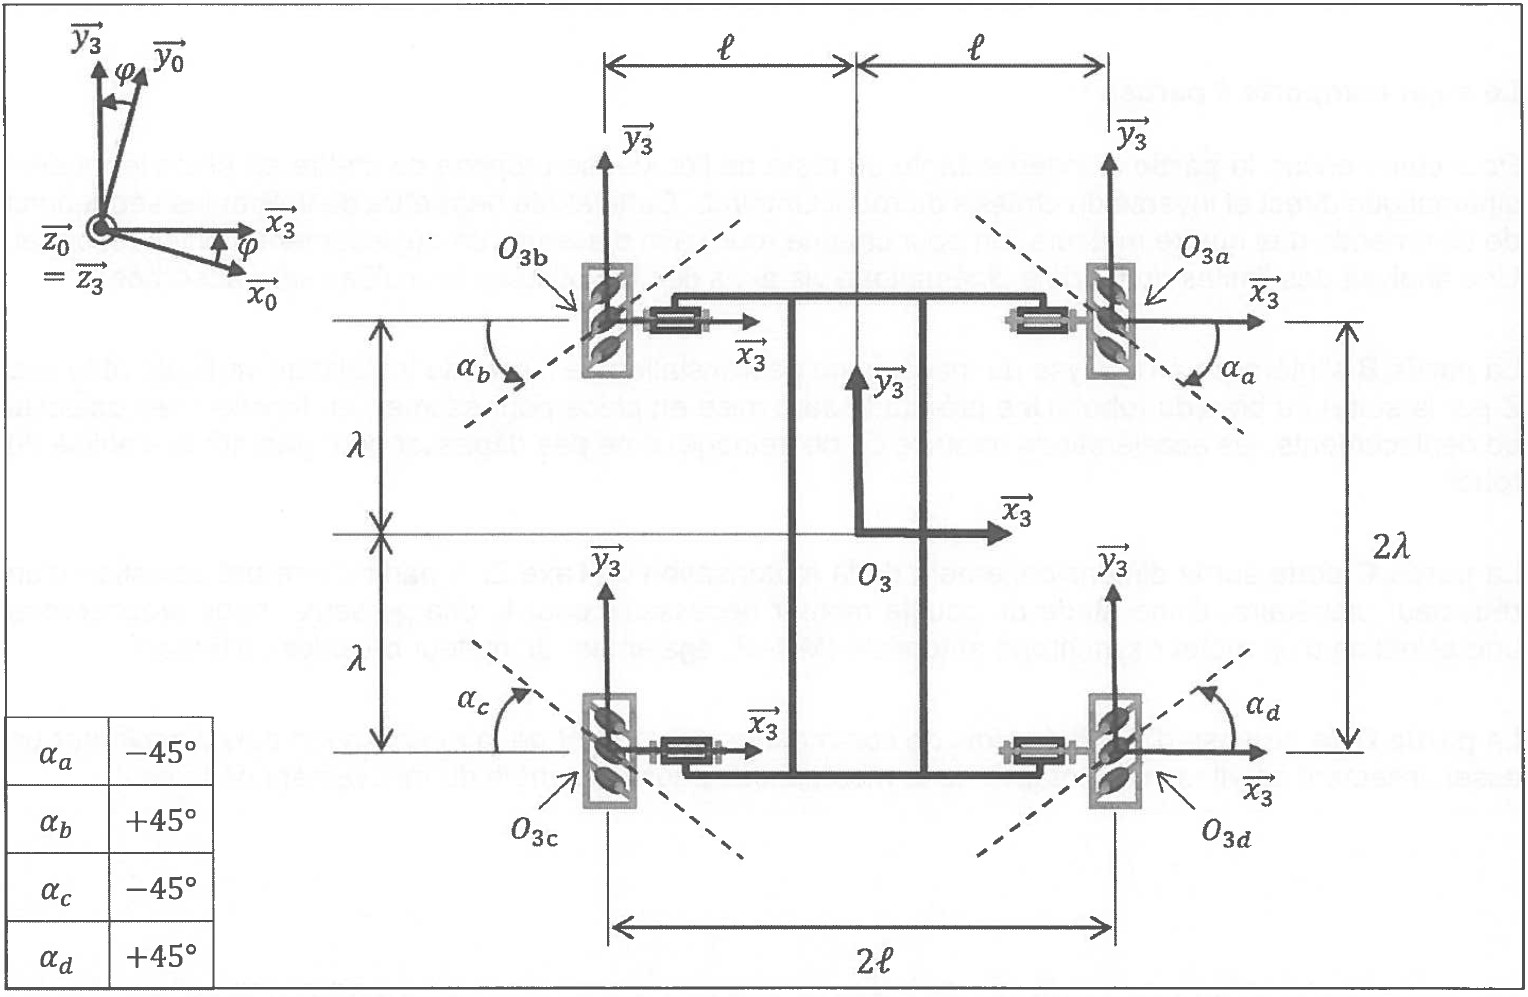
\includegraphics[width=\linewidth]{fig_03}
\end{marginfigure}

\begin{itemize} 
\item On associe le repère $\rep{2}=\repere{A}{x_2}{y_2}{z_2}$ à la tête 2, le repère $\rep{3}=\repere{A}{x_3}{y_3}{z_3}$ à la manivelle 3, le repère $\rep{4}=\repere{B}{x_4}{y_4}{z_4}$ à la bielle 4 et le repère $\rep{5}=\repere{C}{x_2}{y_2}{z_2}$ à la lame 5.
\item La manivelle 3 est en liaison pivot avec la tête 2, d'axe $\axe{A}{y_2}$ et d'angle $\theta_{32}(t)=\angl{x_2}{x_3}=\angl{z_2}{z_3}$.
\item La manivelle 3 est en liaison pivot avec la bielle 4, d'axe $\axe{B}{y_2}$ et d'angle $\theta_{43}(t)=\angl{x_3}{x_4}=\angl{z_3}{z_4}$.
\item La bielle 4 est en liaison pivot avec la lame 5, d'axe $\axe{C}{y_0}$ et d'angle $\theta_{54}(t)=\angl{x_4}{x_2}=\angl{z_4}{z_2}$.
\item La lame 5 est en liaison glissière avec la tête 2, de direction ${z_2}$ et de paramètre linéaire $\lambda(t)$.

\end{itemize}

On pose $\omega_{ij}(t)=\dfrac{\dd \theta_{ij}(t)}{\dd t} = \dot{\theta}_{ij}(t)$, $\vect{AB}=L_3\vect{z_3}$ avec $L_3=\SI{12,5}{mm}$, $\vect{BC}=L_4\vect{z_4}$ avec $L_4=\SI{80}{mm}$ et $\vect{AC}=\lambda(t)\vect{z_2}$.

\question{\label{q17} Déterminer la relation entre les paramètres angulaires $\theta_{32}(t)$, $\theta_{43}(t)$ et $\theta_{54}(t)$.}
\ifprof
\begin{corrige}
\end{corrige}
\else
\fi

\begin{marginfigure}
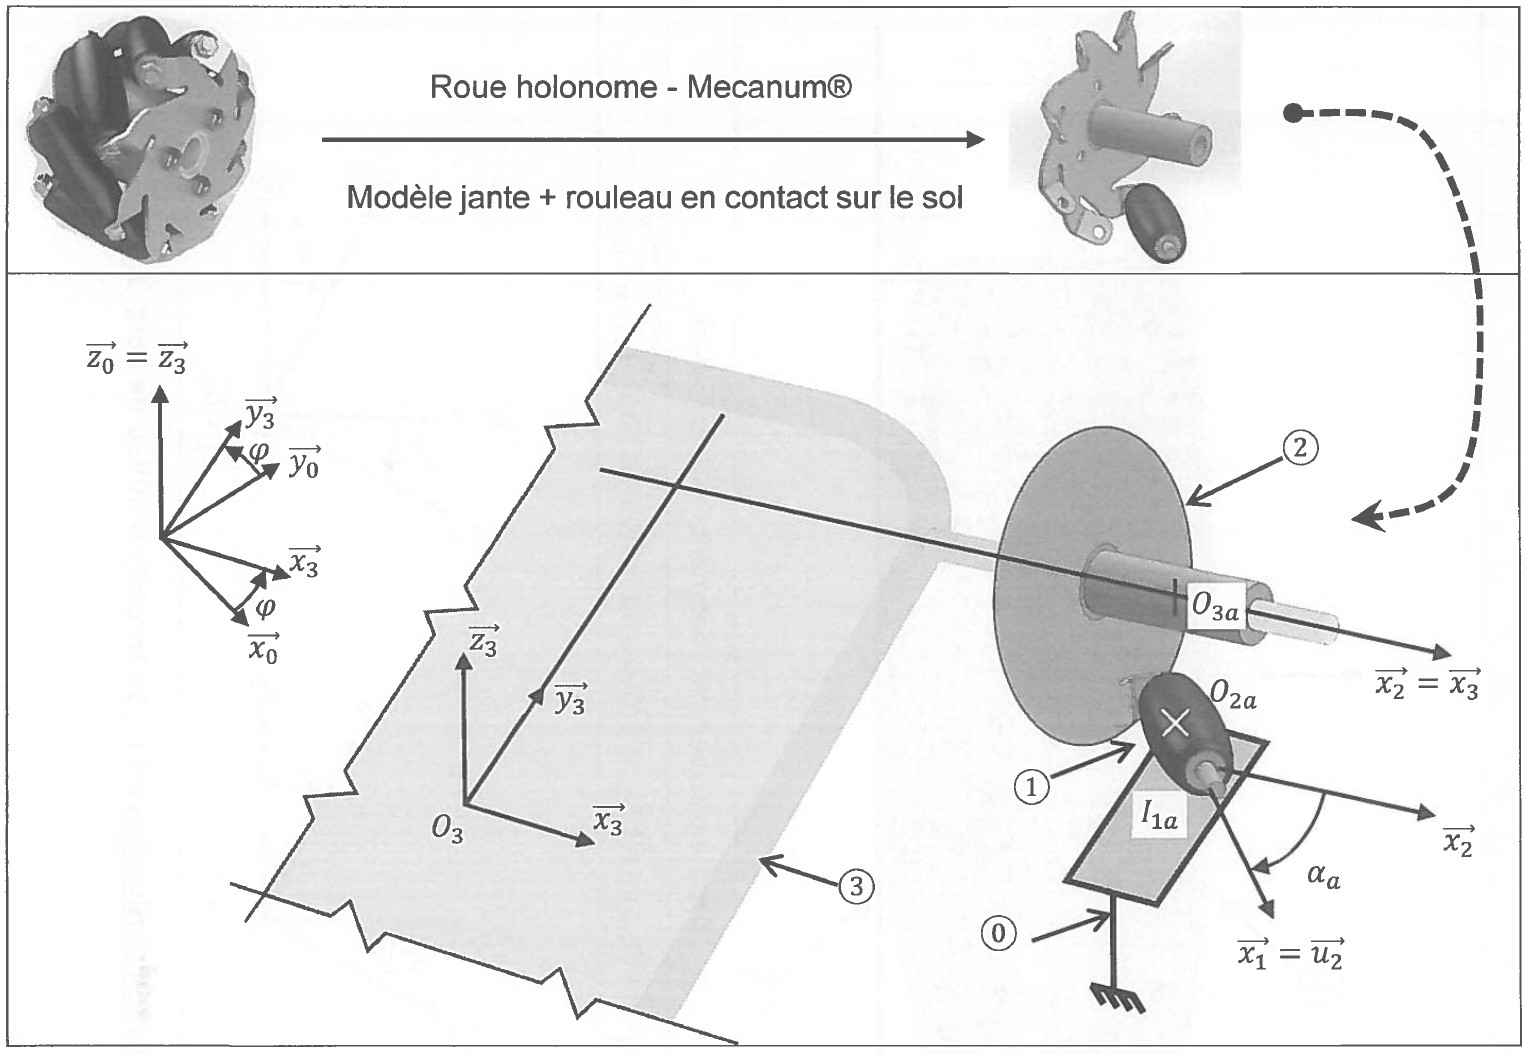
\includegraphics[width=\linewidth]{fig_04}

\caption{Évolution théorique (---) et approximée (- -) du paramètre $\lambda$.}
\end{marginfigure}

\begin{marginfigure}
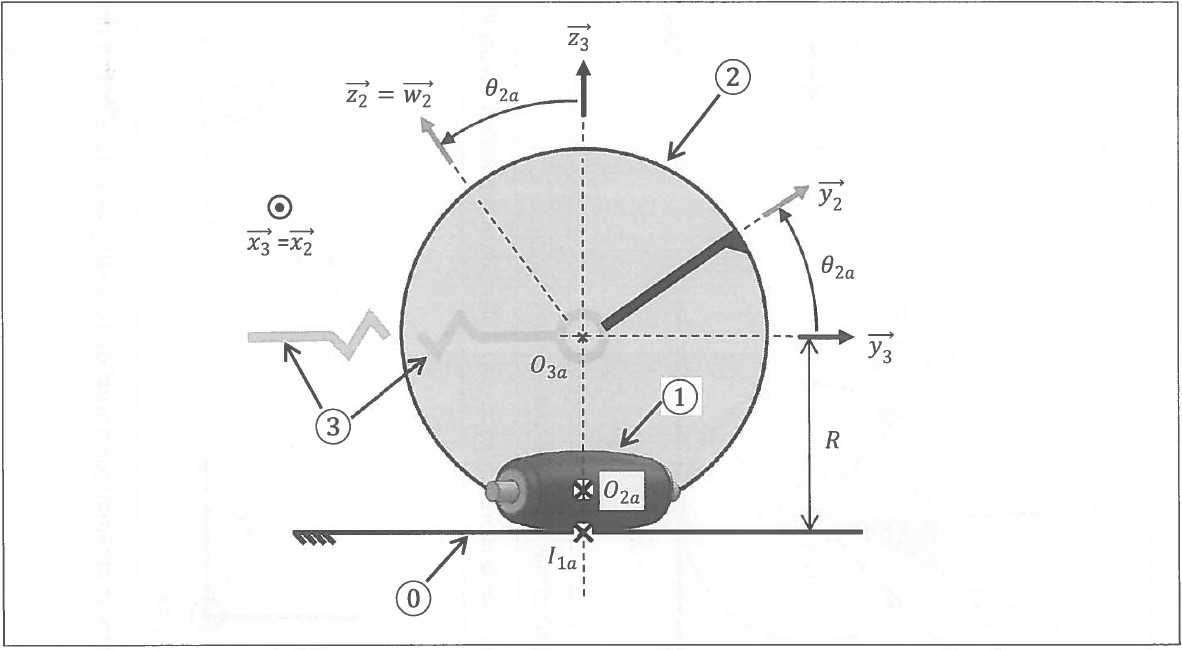
\includegraphics[width=\linewidth]{fig_05}

\caption{Évolution théorique (---) et approximée (- -) de la vitesse  $\dot{\lambda}$ pour $\dot{\theta}_{32}=\SI{3000}{tr.min^{-1}}$.}
\end{marginfigure}


\question{À l’aide d’une fermeture géométrique, déterminer la relation entre le paramètre $\lambda(t)$, l’angle
$\theta_{32}(t)$ et les données géométriques du système.}
\ifprof
\begin{corrige}
\end{corrige}
\else
\fi

\question{En déduire l’expression littérale de l’amplitude des oscillations de la lame, notée $\Delta z$. Faire
l’application numérique et conclure sur le respect de l’exigence 1.2.2.3.}
\ifprof
\begin{corrige}
\end{corrige}
\else
\fi

\question{Calculer le rapport $\left(\dfrac{L_4}{L_3}\right)^2$ et la comparer à la valeur 1. Montrer alors que la loi obtenue à la question \ref{q17} peut se mettre sous la forme $\lambda(t)\simeq L_3 \cos \theta_{32}+L_4$.}
\ifprof
\begin{corrige}
\end{corrige}
\else
\fi

Afin de valider cette approximation, les deux fonctions mathématiques ont été tracées sur un tour de
l’arbre moteur.

\question{Conclure sur l’adoption de la loi approximée dans la suite de l’étude.}
\ifprof
\begin{corrige}
\end{corrige}
\else
\fi


Afin de valider le critère associé à l’exigence de vitesse de coupe, il est nécessaire de déterminer la
loi en vitesse de la lame notée $\dot{\lambda}(t)$.


\ifprof
\else
\begin{marginfigure}
\centering

\includegraphics[width=3cm]{Cy_12_Ch_01_TD_01_Decoupe_qr}
\end{marginfigure}
\fi

\question{Déterminer l’expression littérale de $\dot{\lambda}(t)$ à partir du modèle simplifié de $\lambda(t)$.}
\ifprof
\begin{corrige}
\end{corrige}
\else
\fi

Cette loi en vitesse simplifiée a été tracée sur la figure suivante pour être comparée à la loi obtenue à
partir du modèle établi en question \ref{q17}.



\question{La simplification de la loi en vitesse permet-elle de valider l’exigence 1.2.2.4. ?}
\ifprof
\begin{corrige}
\end{corrige}
\else
\fi
